\documentclass{article}
\usepackage[T1]{fontenc}
\usepackage[polish]{babel}
\usepackage[utf8]{inputenc}
\usepackage[table,xcdraw]{xcolor}
\usepackage[normalem]{ulem}
\usepackage[export]{adjustbox}
\usepackage{lmodern}
\usepackage{fullpage}
\usepackage{longtable}
\usepackage{tikz}
\usetikzlibrary{shapes,arrows,positioning}
\selectlanguage{polish}

\title{Zastosowanie algorytmów sztucznej inteligencji do podejmowania
decyzji na podstawie danych sensorycznych (Reinforcement learning for decission process)} % Title

\author{Dawid Czarneta, Jakub Frąckiewicz, Filip Olszewski, Michał Popiel, Julia Szulc}

\date{\today}


\begin{document}

\maketitle

\section{Cel i zakres dokumentu}
Niniejszy dokument ma za zadanie przedstawić projekt systemu dla inteligentnego domu wykorzystującego uczenie maszynowe (Reinforcement Learning). Projekt ten został stworzony na potrzeby kursu Projekt Zespołowy, na Wydziale Elektroniki Politechniki Wrocławskiej. Dokument ten ma na celu prezentację projektu, przedstawienie jego zakresu, założeń, korzyści, przyczyn uruchomienia, planów zarządzania jakością, ryzykiem jak i komunikacją wewnątrz projektu.

\section{Słownik pojęć}
\begin{tabular}{|l|l|}
\hline
\textbf{Nazwa}                      & \textbf{Wyjaśnienie}                                                                                                                                                                                                                                                                                                                                                                                                                                        \\ \hline
Klient                     & Firma Samsung, pod której opieką merytoryczną tworzony był projekt.                                                                                                                                                                                                                                                                                                                                                                                \\ \hline
Reinforcement Learning, RL & \begin{tabular}[c]{@{}l@{}}Jest to jedna z metod uczenia maszynowego, która polega na wyznaczaniu \\ optymalnej polityki sterowania przez agenta w nieznanym mu środowisku, \\ na podstawie interakcji z tym środowiskiem Jedyną informacją, na której \\ agent się opiera jest sygnał wzmocnienia, który osiąga wysoką wartość\\  (nagrodę), gdy agent podejmuje poprawne decyzje lub niską (karę) gdy\\  podejmuje decyzje błędnie.\end{tabular} \\ \hline
Agent                      & \begin{tabular}[c]{@{}l@{}}Jest to jednostka działająca w środowisku, która na podstawie danych \\ podejmuje właściwe akcje.\end{tabular}                                                                                                                                                                                                                                                                                                          \\ \hline
Środowisko                 & \begin{tabular}[c]{@{}l@{}}Symulacja naturalnego środowiska, stworzona w taki sposób, aby jak \\ najbardziej oddawać rzeczywiste warunki.\end{tabular}                                                                                                                                                                                                                                                                                             \\ \hline
Akcja                      & Jest to realizacja procedur powiązanych z decyzją przez agenta.                                                                                                                                                                                                                                                                                                                                                                                                  \\ \hline
GUI                        & Graficzny interfejs użytkownika.                                                                                                                                                                                                                                                                                                                                                                                                                   \\ \hline
Double DQN                 & \begin{tabular}[c]{@{}l@{}}Double Deep Q Network - algorytm nauki agenta będący rozszerzeniem \\ powszechnie używanego algorytmu Q-Learning.\end{tabular}                                                                                                                                                                                                                                                                                          \\ \hline
\end{tabular}
\section{Cele projektu}

  
Projekt realizuje ideę Reinforcement Learning w procesie decyzyjnym za pomocą niestandardowego agenta oraz środowiska. Celem jest stworzenie działającego systemu dla inteligentnego domu, który analizuje dane zewnętrzne i wewnętrzne zebrane przez czujniki i określa działanie, które należy wykonać, biorąc pod uwagę pożądane przez użytkownika wartości temperatury i światła oraz koszty energii. W rezultacie system powinien minimalizować zużycie energii w domu przy zachowaniu akceptowalnego poziomu komfortu użytkownika.
\section{Zakres i uwarunkowania realizacji}
W projekcie należało zrealizować następujące elementy:
\begin{itemize}
\item Środowisko - należało stworzyć wirtualne środowisko, które ma na celu symulację zewnętrznych warunków pogodowych, dbając przy tym, aby było ono jak najbardziej zbliżone do realistycznych warunków atmosferycznych. Środowisko jest niezbędne do pracy całego systemu, bez dostępu do prawdziwych danych.
\item Agent - główny element całego systemu, to on decyduje o podjęciu konkretnej akcji na podstawie danych zebranych przez sensory oraz preferencji użytkownika. Celem agenta jest jak najlepsze podejmowanie akcji, w celu zminimalizowania zużycia energii przy zachowaniu jak najlepszego komfortu użytkownika.
\item Interfejs dla użytkownika  - należało stworzyć interfejs (tekstowy) dla użytkownika mający na celu przedstawienie przebiegu procesu uczenia przez agenta, jak i możliwość interakcji z systemem, poprzez podawanie własnych akcji, symulując działanie agenta.
\item GUI - graficzny interfejs użytkownika, mający na celu zaprezentować w przystępny sposób działanie agenta w zadanych warunkach środowiska. Wymaganiem co do interfejsu jest to, aby był on jak najbardziej przyjazny dla użytkownika, który nie jest zaznajomiony z systemem i/lub jest to jego pierwsza styczność z systemem.
\end{itemize}

\section{Przyczyny uruchomienia projektu}

Projekt został uruchomiony w formie, która została zaproponowana i dopracowana korzystając ze współpracy z firmą Samsung. Jest to projekt o charakterze badawczym, którego głównym tematem jest zastosowanie algorytmów sztucznej inteligencji do rozwiązywania problemów decyzyjnych na podstawie danych sensorycznych, z wykorzystaniem metod uczenia ze wzmacnianiem (Reinforcement Learning). \\
Główną przyczyną uruchomienia projektu jest rzeczywiste zapotrzebowanie na inteligentne systemy, które stosowane są w inteligentnych domach. Na rynku istnieje duże zapotrzebowanie na oryginalne systemy, które pozwalają na ograniczenie kosztów zużycia energii, co wiąże się  z korzystnym wpływem na środowisko naturalne.

\section{Główne korzyści}
Głównymi korzyściami wynikającymi ze stworzenia inteligentnego systemu, są:
\begin{itemize}
\item Możliwość użycia go podczas tworzenia inteligentnych domów
\item Możliwość implementacji go w istniejących już inteligentnych domach
\item Pozytywny wpływ na środowisko naturalne
\item Oszczędność energii elektrycznej, co w konsekwencji prowadzi do zredukowania kosztów
\item Możliwość osiągnięcia komfortowych warunków dla użytkownika systemu bez konieczności ingerencji użytkownika w działanie systemu
\end{itemize}
\newpage
\section{Wymagania funkcjonalne}
\begin{center}
{\def\arraystretch{3}\tabcolsep=5pt
	\begin{longtable}{p{5cm}p{10cm}}
	
	Pobieranie informacji zebranych przez sensory zewnętrzne&
	\begin{itemize}
	\item \textbf{Przesłanka:} Celem jest dostosowywanie przez system ustawień urządzeń w domu w zależności od warunków zewnętrznych.
	\item \textbf{Kryteria spełnienia:} Zmieniające się warunki pogodowe powinny wpływać na decyzje podejmowane przez system.
	\end{itemize}\\
	
	Pobieranie informacji zebranych przez sensory wewnętrzne&
	\begin{itemize}
	\item \textbf{Przesłanka:} Celem jest dostosowywanie przez system ustawień urządzeń w domu w zależności od warunków wewnętrznych.
	\item \textbf{Kryteria spełnienia:} Zmieniające się warunki w mieszkaniu (temperatura, poziom oświetlenia) powinny wpływać na decyzje podejmowane przez system.
	\end{itemize}\\
	
	Dynamiczny wybór źródła energii, z którego korzysta dom&
	\begin{itemize}
	\item \textbf{Przesłanka:} Celem jest możliwość jak najbardziej ekologicznego zarządzania energią poprzez wykorzystanie ogniw fotowoltaicznych zamiast prądu pobranego z sieci.
	\item \textbf{Kryteria spełnienia:} System powinien wybierać energię z~ogniw fotowoltaicznych wtedy, kiedy to tylko możliwe (kiedy ogniwa nie są rozładowane) zamiast prądu pobranego z sieci.
	\end{itemize}\\
	
	Regulowanie pracy klimatyzacji&
	\begin{itemize}
	\item \textbf{Przesłanka:} Celem jest automatyczne sterowanie klimatyzacją w zależności od temperatury w domu.
	\item \textbf{Kryteria spełnienia:} System powinien mieć możliwość regulowania klimatyzacji w zależności od temperatury zarejestrowanej przez sensory wewnętrzne oraz umieć podjąć jak najlepszą decyzję co do jej ustawień, mając na uwadze koszty energii.
	\end{itemize}\\
	
	Regulowanie ogrzewania&
	\begin{itemize}
	\item \textbf{Przesłanka:} Celem jest automatyczne sterowanie ogrzewaniem elektrycznym w zależności od temperatury w domu.
	\item \textbf{Kryteria spełnienia:} System powinien mieć możliwość regulacji ogrzewania w zależności od zarejestrowanej temperatury w pomieszczeniu oraz podejmować najbardziej optymalną decyzję co do jej ustawień, mając na uwadze koszty energii.
	\end{itemize}\\
	
	Podnoszenie i opuszczanie rolet okiennych&
	\begin{itemize}
	\item \textbf{Przesłanka:} Celem jest automatyczne sterowanie roletami okiennymi w zależności od warunków oświetlenia.
	\item \textbf{Kryteria spełnienia:} System powinien wybrać najdogodniejsze ustawienie rolet w zależności od zarejestrowanych danych na temat oświetlenia zewnętrznego i wewnętrznego.
	\end{itemize}\\

	Sterowanie poziomem oświetlenia&
	\begin{itemize}
	\item \textbf{Przesłanka:} Celem jest automatyczna regulacja natężenia światła w domu w zależności od obecnego poziomu jasności w domu.
	\item \textbf{Kryteria spełnienia:} System powinien mieć możliwość zmiany natężenia światła żarówek w domu w zależności od zarejestrowanego poziomu oświetlenia zarejestrowanego przez sensory wewnętrzne i zewnętrzne.
	\end{itemize}\\

\end{longtable}}
\end{center}

\section{Wymagania niefunkcjonalne}


\subsection{Wymagania estetyczne}
\begin{itemize}
\item \textbf{Wymaganie:} System ma być atrakcyjny dla całej grupy odbiorców
\item \textbf{Kryterium spełnienia:} Reprezentatywna próbka odbiorców ma sama z siebie rozpocząć korzystanie z~systemu.\\
\end{itemize}
\begin{itemize}
\item \textbf{Wymaganie:} System ma wyglądać kompetentnie
\item \textbf{Kryterium spełnienia:} Po pierwszym kontakcie z systemem, 70\% reprezentatywnych potencjalnych nabywców ma się zgodzić ze stwierdzeniem „Czuję, że zaufałbym temu systemowi”.
\end{itemize}

\subsection{Wymagania dotyczące ergonomii i wygody}
\begin{itemize}
\item \textbf{Wymaganie:} System ma być łatwy w użyciu dla całej grupy odbiorców 
\item \textbf{Kryterium spełnienia:} Grupa zaangażowana w testowanie systemu musi być w stanie ukończyć proces uruchomienia i testowania.\\
\end{itemize}
\begin{itemize}
\item \textbf{Wymaganie:} System ma być wykorzystany dla ludzi bez przeszkolenia
\item \textbf{Kryterium spełnienia:} Grupa zaangażowana w testowanie systemu musi być w stanie obsłużyć system, bez wcześniejszego przeszkolenia.\\
\end{itemize}
\begin{itemize}
\item \textbf{Wymaganie:} System ma mieć możliwość regulacji parametrów
\item \textbf{Kryterium spełnienia:} Grupa docelowa musi mieć możliwość regulacji parametrów pracy systemu.\\
\end{itemize}
\begin{itemize}
\item \textbf{Wymaganie:} System ma używać symboli i słów które są naturalnie zrozumiałe dla grupy docelowej użytkowników.
\end{itemize}

\subsection{Wymagania wydajnościowe}
\begin{itemize}
\item \textbf{Wymaganie:} System powinien być dostępny do użytku przez 24 godziny na dobę przez 365 dni w roku.\\
\end{itemize}
\begin{itemize}
\item \textbf{Wymaganie:} System powinien obsługiwać maksymalnie 10 czujników zewnętrznych oraz 10 wewnętrznych.\\
\end{itemize}
\begin{itemize}
\item \textbf{Wymaganie:} System powinien być skalowalny
\item \textbf{Kryterium spełnienia:} Istnieje możliwość dodania dodatkowych czujniuków w każdym momencie działania systemu.\\ 
\end{itemize}
\begin{itemize}
\item \textbf{Wymaganie:} System powinien pracować przez minimum 5 lat bez przekroczenia maksymalnego budżetu zaplanowanego na jego utrzymanie i serwisowanie.\\
\end{itemize}

\subsection{Wymagania dotyczące warunków oraz środowiska pracy}
\begin{itemize}
\item \textbf{Wymaganie:} Produkt ma być używany przez osoby przebywające w domu, przy temperaturze pokojowej.\\
\end{itemize}
\begin{itemize}
\item \textbf{Wymaganie:} Produkt ma umożliwić korzystanie z niego w warunkach słabego oświetlania.\\
\end{itemize}
\begin{itemize}
\item \textbf{Wymaganie:} Produkt nie może emitować dźwięków.
\end{itemize}

\subsection{Wymagania dotyczące utrzymania i wsparcia}
\begin{itemize}
\item \textbf{Wymaganie:} Nowe czujniki powinny zostać oddane do systemu w ciągu maksymalnie jednego dnia pracy.\\
\end{itemize}
\begin{itemize}
\item \textbf{Wymaganie:} System powinien zapewniać wsparcie dla klienta w razie problemów z jego użytkowaniem.\\
\end{itemize}

\subsection{Wymagania bezpieczeństwa}
\begin{itemize}
\item \textbf{Wymaganie:} System ma być zabezpieczony przed wprowadzeniem niewłaściwych danych.\\
\end{itemize}
\begin{itemize}
\item \textbf{Wymaganie:} System ma się sam bronić przed zamierzonym wykorzystaniem niezgodnie z przeznaczeniem.\\
\end{itemize}

\subsection{Wymagania kulturowe i polityczne}
\begin{itemize}
\item \textbf{Wymaganie:} Produkt powinien zapewniać możliwość używania danych jednostek temperatury w zależności od lokalizacji w jakiej jest używany.\\
\end{itemize}

\section{Koszty}
Projekt ze względu na to, że jest projektem akademickim, jak i jego stworzenie nie wymagało zakupu sprzętu czy też oprogramowania, nie wygenerował żadnych kosztów. Wszystkie materiały jakie zostały wykorzystane przy tworzeniu systemu, były udostępnione bezpłatnie i zostały użyte zgodnie z ich licencją.

\section{Terminy}
Terminarz projektu można podzielić na dwie części:
\begin{itemize}
\item Przygotowywanie dokumentacji projektowej
\item Przygotowywanie systemu (planowanie, implementacja, testy)
\end{itemize}\mbox{}\\
Terminy przygotowywania dokumentacji projektowej:
\begin{itemize}
\item Wybranie tematu projektu oraz zgłoszenie składu grupy - 9.03.2018
\item Specyfikacja wymagań funkcjonalnych - 23.03.2018
\item Struktura organizacyjna i plan komunikacji w projekcie - 13.04.2018
\item Projekt zarządzania jakością - 27.04.2018
\item Zarządzanie ryzykiem - 18.05.2018
\item Dokumentacja projektu - 6.06.2018
\end{itemize}\mbox{}\\
Terminy przygotowywania systemu:
\begin{itemize}
\item Określenie terminów organizacyjnych takich spotkania zespołu, rozmowy z opiekunem projektu - 28.02.2018
\item Projekt szkieletu klas aplikacji - 13.03.2018
\item Projekt funkcji nagrody otrzymywanej przez agenta - 13.03.2018
\item Stworzenie diagramu klas - 15.03.2018
\item Implementacja akcji możliwych do wykonania przez agenta  - 19.03.2018
\item Implementacja funkcji nagrody otrzymywanej za podejmowanie akcji - 20.03.2018
\item Projekt szkieletu klasy agenta - 25.03.2018
\item Ustalenie i implementacja zależności wewnętrznych - 24.03.2018
\item Przygotowanie spisu konwencji na temat kodu źródłowego aplikacji - 4.04.2018
\item Implementacja podstawowej wersji agenta - 18.04.2018
\item Stworzenie zależności pogodowych w środowisku - 18.04.2018
\item Dokumentacja na temat algorytmów używanych w agencie - 19.04.2018
\item Manualne testy działania środowiska - 20.04.2018
\item Zapisywanie i wczytywanie modeli sieci neuronowej agenta - 25.04.2018
\item Analiza i testy rozwiązań chmurowych służących do przyspieszenia obliczeń - 8.05.2018
\item Implementacja konsolowego interfejsu użytkownika - 8.05.2018
\item Implementacja Double DQN - 8.05.2018
\item Stworzenie plików konfiguracyjnych do przechowywania parametrów Agenta - 14.05.2018
\item Projekt i wymagania funkcjonalne GUI - 4.05.2018
\item Implementacja GUI - 21.05.2018
\item Omówienie i przedstawienie systemu 11.06.2018
\end{itemize}


\section{Plan i produkty projektu}
Plan projektu składa się z następujących etapów:
\begin{itemize}
\item Działania badawcze - etap polegający na zapoznaniu się z problemem oraz sposobami i alogrytami rozwiązującymi problem, teoretyczne zapoznanie się z bibliotekami i narzędziami, używanymi w kolejnych etapach tworzenia systemu.
\item Planowanie - etap, w którym został stworzony koncept systemu, wstępny podział prac oraz harmonogram
\item Implementacja rozwiązań - na tym etapie zostały zaimplementowane wybrane podczas planowania algorytmy
\item Testy działania systemu - system został przetestowany w celu sprawdzenia, czy zachowuje się w oczekiwany sposób
\item Poprawa działania systemu - poprzez odpowiedni dobór parametrów, system został ulepszony w celu osiągnięcia najlepszych rezultatów
\end{itemize} \mbox{}\\
Produktami projektu są: \mbox{}\\
Aplikacja - systemu dla inteligentnego domu, w którym zawarty jest:
\begin{itemize}
\item Stworzony agent
\item Środowisko
\item Interfejs użytkownika
\item GUI
\end{itemize} \mbox{}\\
Dokumentacja projektowa - dokument zawierający:
\begin{itemize}
\item Cele projektu
\item Słownik pojęć
\item Zakres i uwarunkowania realizacji projektu
\item Przyczyny uruchomienia projektu
\item Główne korzyści wynikające z projektu
\item Koszty, terminy
\item Plan i produkty projektu
\item Strukturę organizacyjną i zakres odpowiedzialności w projekcie
\item Harmonogram
\item Plan komunikacji w projekcie
\item Plan zarządzania jakością
\item Plan zarządzania ryzykiem
\end{itemize} \mbox{}\\
Dokumentacja techniczna dla firmy Samsung - dokument zawierający:
\begin{itemize}
\item Ideę projektu
\item Cel projektu
\item Zrzuty ekranu prezentujące wygląd systemu
\item Opis zrealizowanych funkcjonalności
\item Opis metody Reinforcement Learning
\item Opis użytych bibliotek - w szczególności PyTorch
\item Sposób uruchamiania systemu
\item Sposób korzystania z systemu
\item Opis testów systemu
\item Opis środowiska - działanie, sposób generowania pogody i funkcji nagrody
\item Dokładny opis agenta - użytych algorytmów oraz sposobów implementacji agenta w innym środowisku
\item Opis plików konfiguracyjnych
\item Opis nieudanych rozwiązań
\item Opis wpływu parametrów na działanie uczenia agenta
\item Wnioski i opis wiedzy zdobytej podczas tworzenia systemu
\item Potencjalne kierunki rozwoju projektu
\end{itemize}

\section{Struktura organizacyjna i zakresy odpowiedzialności}
\subsection{Struktura organizacyjna}
Podczas pracy przyjęliśmy ogólny podział obowiązków między osoby w zespole:

\begin{itemize}
\item Filip Olszewski - lider zespołu, specjalista z tematyki uczenia maszynowego, programista
\item Michał Popiel - ekspert z dziedziny Pythona, optymalizacji kodu, programista
\item Julia Szulc - zarządzanie kodem w serwisie GitHub, programista
\item Dawid Czarneta - zarządzanie zadaniami w Trello, programista
\item Jakub Frąckiewicz - tester integralności systemu, programista
\end{itemize}
Lecz obowiązki wynikające z aktualnych zadań przydzielane są co tydzień. Jako, że jako cały zespół chcemy dobrze znać tworzony system, dzielimy się obowiązkami w~taki sposób, aby każdy miał swój udział w~pisaniu  kluczowych modułów systemu oraz w~stworzeniu do nich testów.
Dokumentacja w projekcie jest przygotowywana wspólnie przez cały zespół.

% Define block styles
\tikzstyle{block} = [rectangle, draw, fill=blue!20, 
    text width=10em, text centered, rounded corners, minimum height=4em]
\tikzstyle{line} = [draw, -latex']
    
\newpage
\subsection{Diagram organizacyjny}
\begin{center}
\begin{tikzpicture}[node distance = 2.5cm, auto]
    % Place nodes
    \node [block, fill=none] (leader) {Lider zespołu};
    \node [draw=none, fill=none, below of=leader] (hidden) {};     
    \node [block, right of=hidden, node distance = 6cm, fill=none] (opiekun) {Opiekun z firmy Samsung}; 
    \node [block, below of=hidden, fill=none] (tester) {Tester systemu};
    \node [block, left of=tester, node distance = 6cm, fill=none] (project_manager) {Menadżer projektu};
    \node [block, below of=project_manager, fill=none] (repository_manager) {Menadżer repozytorium kodu};
    \node [block, below of=repository_manager, fill=none] (programmer) {Programista};
    \node [block, right of=tester, node distance = 6cm, fill=none] (doc_creator) {Twórca dokumentacji};

	% Coordinates to draw lines
	\node [coordinate, below = 1cm of hidden] (C1){};
    \node [coordinate, right = 6cm of C1] (R1){};
    \node [coordinate, below = 0.7cm of R1] (B1){};
    \node [coordinate, left = 6cm of C1] (L1){}; 
    \node [coordinate, below = 0.7cm of C1] (B2){};  
    \node [coordinate, below = 0.7cm of L1] (B3){};    
    
    % Draw edges
    \path [line] (opiekun) -- (hidden);
    \path [line] (leader) -- (B2);
    \path [line] (C1) -| (B1);
    \path [line] (C1) -| (B3);
    \path [line] (project_manager) -- (repository_manager);
    \path [line] (repository_manager) -- (programmer);


\end{tikzpicture}
\end{center}
\section{Harmonogram}

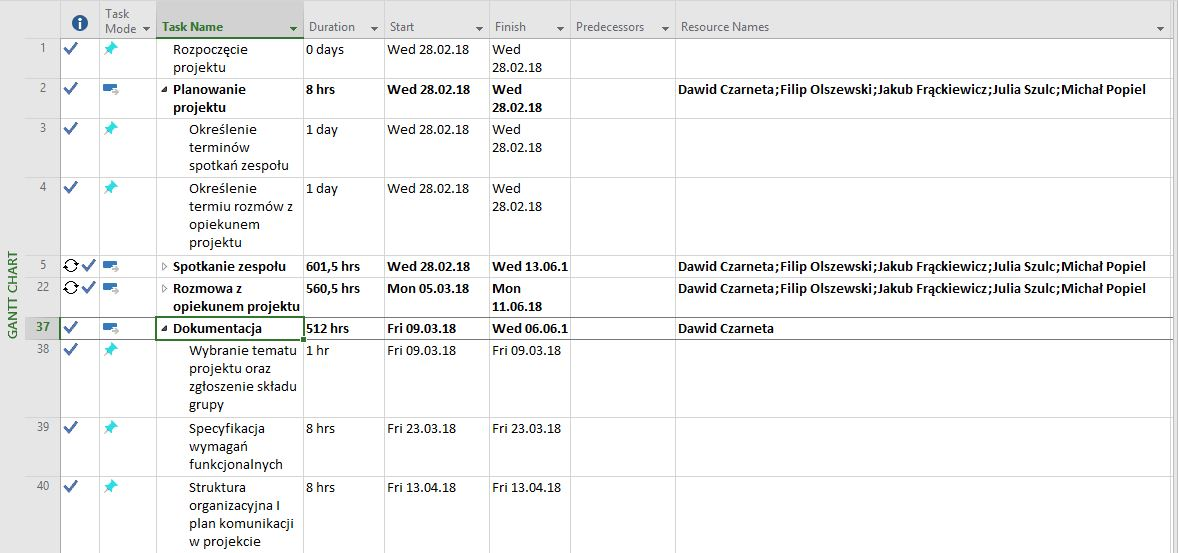
\includegraphics[width=1\textwidth, left]{final/1.JPG}
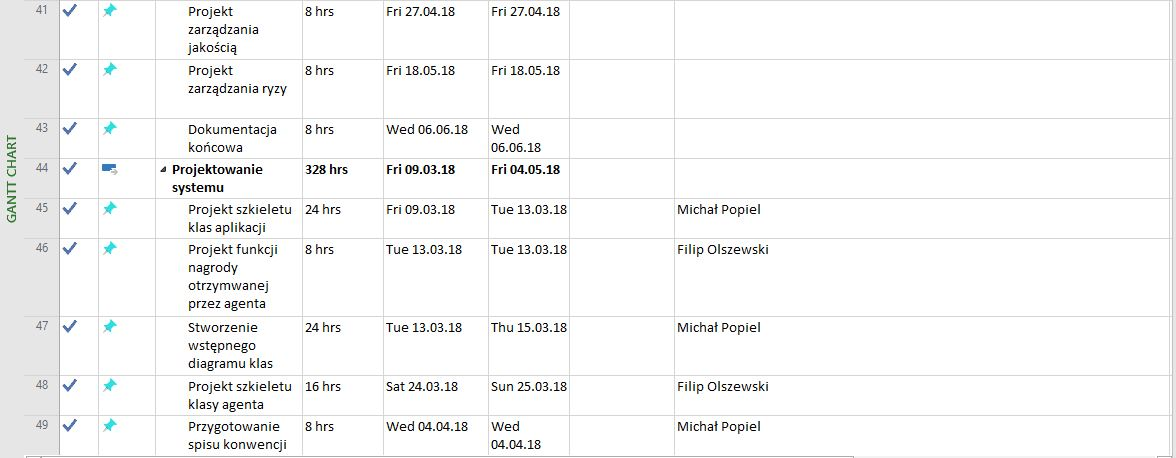
\includegraphics[width=1\textwidth, left]{final/2.JPG}
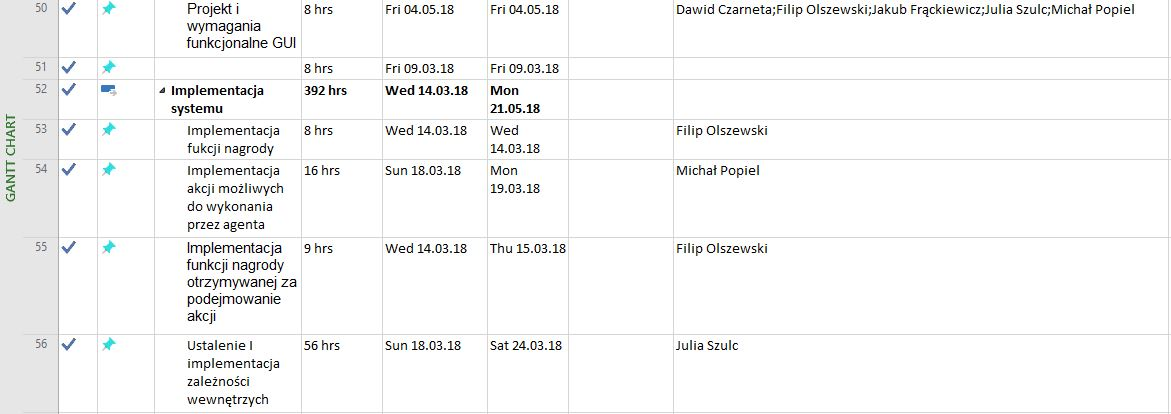
\includegraphics[width=1\textwidth, left]{final/3.JPG}
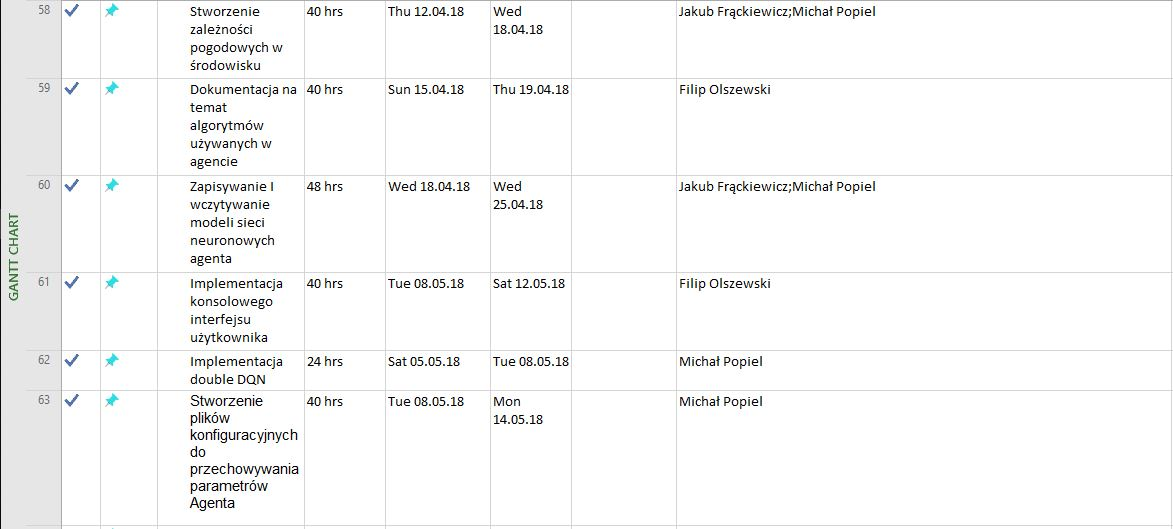
\includegraphics[width=1\textwidth, left]{final/4.JPG}
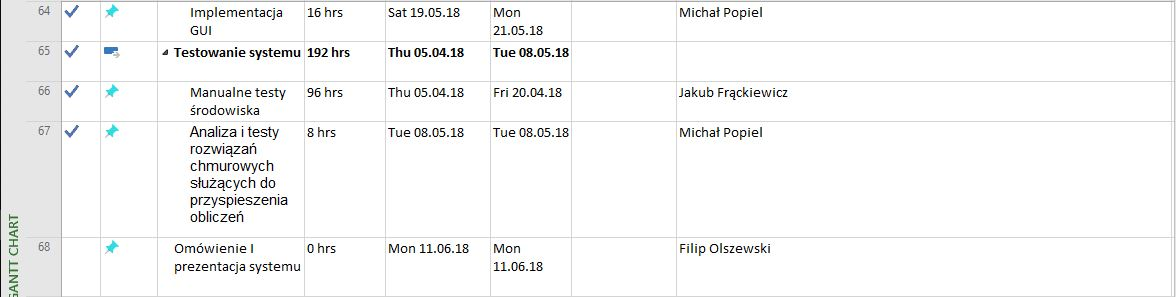
\includegraphics[width=1\textwidth, left]{final/5.JPG}

\section{Plan komunikacji}
Praca przy projekcie odbywa się z wykorzystaniem systemu Kanban. W każdym tygodniu pracy odbywa się spotkanie zespołu, na którym omawiane są postępy, rozwiązywane problemy jak i przygotowywane następny zadania. Raz w tygodniu odbywa się również wideokonferencja zespołu z opiekunem projektu z~ramienia firmy Samsung, na którym omawiane są postępy w~tworzeniu systemu jak i konsultowane są problemy techniczne, które występują w czasie wytwarzania oprogramowania. 
Na każdym ze spotkań tworzone są notatki, które następnie wykorzystywane są jako protokół ze spotkania, aby wszyscy członkowie zespołu mieli wgląd i jasność co do ustaleń wynikających ze spotkania. \mbox{}\\
Do zarządzania zadaniami \nobreak używane jest narzędzie Trello (do zarządzania tablicą zadań), gdzie dla każdego etapu pracy przygotowana jest \nobreak odpowiednia kolumna. Każde większe zadanie lub funkcjonalność na początku jest planowana, następnie zostaje zdekomponowana na jak najmniejsze zadania w celu umożliwienia podziału ich na członków zespołu. \nobreak Następnie zadania te wpisywane są do narzędzia Trello, i przypisywane są do niego wybrane osoby. Następnie osoby te pracują nad zadaniami (przenosząc je odpowiednio na odpowiednie kolumny na tablicy Kanban, kiedy zadanie to spełnia założenia Definition of Done). Gdy praca nad zadaniem zostanie zakończona przenoszone jest ono do kolumny “Review”, po spełnieniu DoD, które w tym przypadku polega na stworzeniu konkretnego efektu pracy w postaci kodu, diagramu lub opisu słownego. Jeżeli efektem pracy jest kod, muszą być stworzone do tego kodu testy jednostkowe. Następnie po przejrzeniu i zaakceptowaniu efektów pracy przez wszystkich członków zespołu, zadanie to zostaje przeniesione do kolumny “Zrobione”, gdzie jest ono uznawane za oficjalnie zakończone. Część z zadań oznaczana jest jako “zależne od”, co oznacza, że aby rozpocząć wybrane zadanie należy najpierw ukończyć zadanie poprzednie, od którego to zadanie jest zależne. \\
Do wersjonowania kodu używany jest system kontroli wersji Git, a kod przechowywany jest w serwisie \nobreak GitHub.

\section{Plan jakości}
\subsection{Założenia teoretyczne projektu zarządzania jakością}
Pojęcie jakości w projekcie postrzegane jest jako zgodność rezultatu projektu ze
specyfikacjami, przeznaczeniem i oczekiwaniami odbiorcy.
Zarządzanie jakością w projekcie obejmuje procesy zarządzania jakością jak i techniki których celem jest obniżenie ryzyka związanego z niedotrzymaniem wymogów przez końcowy efekt projektu. Proces zarządzania jakością w projekcie składa się z etapów:
\begin{itemize}
\item Planowania jakości
\item Zapewniania jakości
\item Kontroli jakości
\end{itemize}

\subsection{Oczekiwania jakościowe odbiorcy projektu}

Odbiorca, czyli firma Samsung oczekuje od projektu, aby był on stworzony zgodnie z najwyższą jakością oraz w pełni przetestowany (zarówno jednostkowo jak i integracyjnie). Wyznacza również terminy realizacji kolejnych wersji systemu, po których następuje faza weryfikacji i akceptacji według zdefiniowanych kryteriów.

\subsection{Wymagania jakościowe dla każdej z ról w projekcie}
    
Każdy członek zespołu pełni rolę odbiorcy prac od innych członków zespołu jak i dostarczyciela wysokiej jakości produktu dla współpracowników, którzy przejmują jego pracę. Na każdym z etapów tworzenia systemu, każdy z członków zespołu powinien informować o statusie wykonywania pracy oraz o ewentualnych problemach w trakcie ich wykonywania.\\
Lider zespołu odpowiada za wdrożenie i utrzymanie zarządzania jakością w projekcie jak i raportowaniem danych związanych ze wskaźnikami jakościowymi. Jest on odpowiedzialny również za techniczną spójność dokumentów, ich zgodność ze standardami jakości oraz za zapewnienie wysokiej jakości produktów.\\
Osoby do których skierowany jest projekt są odpowiedzialne za ustalanie kierunku prac, decyzje w sprawie ogólnych celów projektu.\\
Zadaniem osoby z ramienia uczelni (w przypadku naszego projektu, prof. Michał Woźniak) jest odpowiedzialna za odbiór i weryfikację tworzonych dokumentów projektowych oraz przestrzeganie terminów weryfikacji i akceptacji.

\subsection{Wymagania jakościowe dla zadań w projekcie}

W projekcie w celu utrzymania wysokiej jakości systemu zostały zdefiniowane reguły akceptacji na każdym z etapów pracy projektowej. \\
Dla zadań związanych z tworzeniem dokumentacji, po przygotowaniu danego etapu, każdy z członków zespołu musi się z nim zapoznać, oraz zgłosić ewentualne uwagi. Następnie zadanie to jest przekazywane do prof. Woźniaka w celu weryfikacji, następnie, gdy zostaną zgłoszone uwagi, zadanie to trafia do poprawy i~po poprawie, zadanie jest wysyłane i uznawane za zakończone. \\
Każde zadanie związane z tworzeniem kodu systemu również posiada kryteria jakości, takie jak testy jednostkowe oraz manualne sprawdzenie działania stworzonej w ramach tego zadania funkcjonalności. Następnie taki kod przechodzi przez etap Code Review przez pozostałych członków zespołu, nieuczestniczących bezpośrednio przy danym zadaniu.\\
Regularnie odbywają się również testy integracyjne całego systemu, aby mieć pewność, że działa on bez zarzutów.
\mbox{}\\\mbox{}\\\mbox{}\\
W projekcie został stworzony również dokument odpowiedzialny za kod źródłowy systemu. Opisane są w~nim szczegółowo konwencje na temat
\begin{itemize}
\item formatowania kodu
\item tworzenia komentarzy
\item tworzenia dokumentacji
\item projektowania i tworzenia testów
\item nazewnictwa zmiennych i metod
\item pracy z systemem kontroli wersji (nazewnictwo commitów i branchy)
\end{itemize}



\section{Zarządzanie ryzykiem}

\subsection{ Planowanie zarządzania ryzykiem}
\mbox{}\\
Ryzyko to prawdopodobieństwo wystąpienia sytuacji, która może oddziaływać na dalszy przebieg projektu- jego jakość, zakres, koszty i/lub harmonogram.
Zarządzanie ryzykiem jest bardzo ważnym elementem każdego projektu, które polega na monitorowaniu i obniżaniu ryzyka projektu do poziomu akceptowalnego przez menadżera projektu.
W planie zarządzania projektem należy zdefiniować wstępną ocenę skutków wystąpienia ryzyka, oraz wstępną ocenę prawdopodobieństwa wystąpienia takiego zdarzenia.
\mbox{}\\
Wstępna ocena skutków wystąpienia ryzyka – wstępna ocena skutków wystąpienia danego ryzyka została sklasyfikowana opisowo, według następującego klucza:
\begin{itemize}
\item{Niskie}
\item{Średnie}
\item{Wysokie}
\end{itemize}
Wstępna ocena prawdopodobieństwa – wstępna ocena skutków wystąpienia danego ryzyka została sklasyfikowana opisowo, według następującego klucza:
\begin{itemize}
\item{Mało prawdopodobne (0 – 20\%)}
\item{Możliwe (20\% - 60\%)}
\item{Prawdopodobne (60\% - 100\%)}
\end{itemize}
Każdy z członków zespołu odpowiedzialny jest za kontrolę i dbałość o jakość projektu, w celu uniknięcia wystąpienia ryzyka.  
Na każdym z etapów projektu należy przeprowadzić kontrolę ryzyka, poprzez porównanie wyników prac z możliwymi przypadkami zdefiniowanymi w formularzach analizy ryzyka, należy zwrócić uwagę również na inne, nie ujęte w formularzach sytuację, i w razie stwierdzenia, że jest to sytuacja zidentyfikowana jako ryzyko, należy po uzgodnieniu z liderem projektu zaktualizować lub dodać kolejny formularz analizy ryzyka. 
Progi akceptacji czyli kryteria określające, kiedy powinny zostać podjęte działania będące odpowiedzią na zaistniałe ryzyko, ustalane są przez wszystkich członków zespołu.

\subsection{Identyfikacja ryzyka}
\mbox{}\\
W procesie tym występuje wykrycie źródeł ryzyka, a następnie ich usystematyzowanie według przyjętych kategorii. Po przeprowadzeniu analizy, zostały stworzone następujące kategorie źródeł ryzyka:

\begin{enumerate}
\item{Strategiczne i handlowe}
	\begin{enumerate}
		\item{Dodawanie nowych wymagań po zamknięciu specyfikacji}
		\item{Nieczytelność serwisu}
	\end{enumerate}
\item{Ekonomiczne, finansowe i rynkowe}
	\begin{enumerate}
		\item{Niemożność ukończenia projektu ze względu na brak finansów}
	\end{enumerate}
\item{Organizacyjne, zarządzania i związane z czynnikiem ludzkim}
	\begin{enumerate}
		\item{Błędnie stworzona specyfikacja systemu}
		\item{Utrudnienia w komunikacji}
		\item{Choroby, wypadki}
		\item{Niedoświadczony zespół}
		\item{Nieodpowiedni kierownik zespołu}
	\end{enumerate}
\item{Techniczne, operacyjne i związane z infrastrukturą}
	\begin{enumerate}
		\item{Utrata danych}
		\item{Wybór nieodpowiednich technologii do realizacji systemu}
		\item{Błędy w implementacji systemu}
	\end{enumerate}
\end{enumerate}

\subsection{Jakościowa analiza ryzyka}
Analiza skutków wystąpienia ryzyka, w kolejności od krytycznych do mających najmniejszy wpływ na projekt:
\begin{enumerate}
\item{Utrata danych}
\item{Błędnie stworzona specyfikacja projektu}
\item{Dodawanie nowych wymagań po zamknięciu specyfikacji}
\item{Wybór nieodpowiednich technologii do realizacji systemu}
\item{Błędy w implementacji systemu}
\item{Choroby/wypadki}
\item{Niedoświadczony zespół}
\item{Nieodpowiedni kierownik zespołu}
\item{Niemożność ukończenia projektu ze względu na brak finansów}
\item{Utrudnienia w komunikacji}
\item{Nieczytelność serwisu}
\end{enumerate}

\subsection{Ilościowa analiza ryzyka}
Oszacowanie wagi dla każdego ryzyka na podstawie prawdopodobieństwa wystąpienia, oraz wpływu na projektu
Obliczane według następującego wzoru (skutek\_ryzyka \* prawd\_wystąpienia)
\mbox{}\\\mbox{}\\
Wagi dla skutków ryzyka
\begin{itemize}
\item{Niskie     - Waga: 1}
\item{Średnie    - Waga: 2}
\item{Wysokie	 - Waga: 3}
\end{itemize}
\mbox{}\\
\mbox{}\\
Wagi dla prawdopodobieństw wystąpienia
\begin{itemize}
\item{Mało prawdopodobne (0 – 20\%) - Waga: 1}
\item{Możliwe (pow. 20\% - 60\%) - Waga: 2}
\item{Prawdopodobne (pow. 60\% - 100\%) - Waga: 3}
\end{itemize}
\mbox{}\\ \mbox{}\\
Źródła ryzyka wraz z wagami prezentują się następująco:
\begin{enumerate}
\item{Utrata danych - (3*2) = 6}
\item{Błędnie stworzona specyfikacja projektu - (3*2) = 6}
\item{Dodawanie nowych wymagań po zamknięciu specyfikacji - (3*1) = 3}
\item{Wybór nieodpowiednich technologii do realizacji systemu - (3*2) = 6}
\item{Błędy w implementacji systemu - (3*2) = 6}
\item{Choroby/wypadki - (3*1) = 3}
\item{Niedoświadczony zespół - (3*2) = 6}
\item{Nieodpowiedni kierownik zespołu - (3*1) = 3}
\item{Niemożność ukończenia projektu ze względu na brak finansów - (3*1) = 3}
\item{Utrudnienia w komunikacji - (1*1) = 1}
\item{Nieczytelność serwisu - (1*1) = 1}
\end{enumerate}
\newpage
\subsection{Planowanie reakcji na ryzyko}
\mbox{}\\ \mbox{}\\
%\begin{table}[]
%\centering
%\caption{My caption}
\hspace*{-0.9cm}
\label{my-label}
\begin{tabular}{|l|l|l|}
\hline
\rowcolor[HTML]{C0C0C0} 
Zagrożenie                                                                                            & Strategia  & Środki zaradcze                                                                                                                                                                                                                         \\ \hline
\begin{tabular}[c]{@{}l@{}}Dodawanie nowych wymagań po\\ zamknięciu specyfikacji\end{tabular}         & Redukcja   & \begin{tabular}[c]{@{}l@{}}Upewnienie się, że lista wymagań  jest kompletna jeszcze przed\\  zamknięciem specyfikacji\end{tabular}                                                                                                       \\ \hline
Nieczytelność serwisu                                                                                 & Redukcja   & Konsultacje z klientem, w celu akceptacji wyglądu aplikacji                                                                                                                                                                             \\ \hline
\begin{tabular}[c]{@{}l@{}}Niemożność ukończenia projektu ze \\ względu na brak finansów\end{tabular} & Redukcja   & \begin{tabular}[c]{@{}l@{}}Przeanalizowanie serwisów, w celu znalezienia najtańszego\\  lub darmowego rozwiązania\end{tabular}                                                                                                          \\ \hline
Błędnie stworzona specyfikacja systemu                                                                & Redukcja   & \begin{tabular}[c]{@{}l@{}}Konsultacje z ekspertem ze strony klienta,  konsultacje\\ z osobami doświadczonymi w temacie projektu, udzielanie\\  się na forach dyskusyjnych, związanych  z używaną\\ w systemie technologią\end{tabular} \\ \hline
Utrudnienia w komunikacji                                                                             & Redukcja   & Zapewnienie nadmiarowej ilości kanałów komunikacyjnych                                                                                                                                                                                  \\ \hline
Choroby, wypadki                                                                                      & Akceptacja & \begin{tabular}[c]{@{}l@{}}Każdy członek zespołu powinien być samodzielny, by być\\  w stanie przejąć obowiązki i zadania  od innego członka zespołu.\end{tabular}    \\ \hline
Niedoświadczony zespół                                                                                & Redukcja   & \begin{tabular}[c]{@{}l@{}}Przeprowadzenie szkolenia przez eksperta z danej technologii,\\   samokształcenie się przez wszystkich członków zespołu\\   z oficjalnej dokumentacji\end{tabular}                                             \\ \hline
Nieodpowiedni kierownik zespołu                                                                       & Redukcja   & \begin{tabular}[c]{@{}l@{}}Sprawdzenie kompetencji osoby, która ma zostać kierownikiem\\ zespołu\end{tabular}                                                                                                                          \\ \hline
Utrata danych                                                                                         & Redukcja   & \begin{tabular}[c]{@{}l@{}}Należy osiągnąć nadmiarowość danych  za pomocą kopii\\ zapasowych\end{tabular}                                                                                                                               \\ \hline
\begin{tabular}[c]{@{}l@{}}Wybór nieodpowiednich technologii\\ do realizacji systemu\end{tabular}     & Redukcja   & \begin{tabular}[c]{@{}l@{}}Dokładna analiza dostępnych technologii przed  przystąpieniem\\ do projektowania systemu\\ \\ Projekt systemu w możliwie jak najbardziej niezależny od \\  technologii sposób\end{tabular}                    \\ \hline
Błędy w implementacji systemu                                                                         & Redukcja   & \begin{tabular}[c]{@{}l@{}}Testy systemu na każdym etapie tworzenia\\ \\ Konsultacje z ekspertem w celu weryfikacji zastosowanych\\ rozwiązań\end{tabular}                                                                          \\ \hline
\end{tabular}
%\end{table}
\mbox{}\\\mbox{}\\
\subsection{Monitorowanie i kontrolowanie ryzyka}
\mbox{}\\
W celu monitorowania i kontroli ryzyka, na każdym etapie należy analizować i śledzić ryzyka, które występują w projekcie, oraz zajmować się rozpatrywaniem nowego ryzyka. Należy również analizować skuteczność działań podejmowanych jako reakcja na ryzyko. W projekcie osobą odpowiedzialną jest kierownik projektu, oraz w celu weryfikacji jego pracy inny członek zespołu, wyznaczony w celu kontroli i weryfikacji błędów.


\mbox{}\\\mbox{}\\\mbox{}\\\mbox{}\\\mbox{}\\\mbox{}\\\mbox{}\\
\subsection{Formularze analizy ryzyka}
\mbox{}\\\mbox{}\\
\newcolumntype{L}[1]{>{\raggedright\arraybackslash}p{#1}}

{\def\arraystretch{1.3}\tabcolsep=10pt
\begin{tabular}{|L{6cm}|L{9cm}|}
\hline
Formularz analizy ryzyka &  \\
\hline
Ryzyko 						   & \textbf{Dodawanie nowych wymagań po zamknięciu specyfikacji} \\
\hline
Opis zagrożenia				   & Dodawanie nowych wymagań może spowodować przekroczenie harmonogramu orazpotrzebę modyfikacji wymagań już istniejących \\
\hline
Prawdopodobieństwo wystąpienia & Mało prawdopodobne \\
\hline
Wpływ na realizację projektu   & Wysoki \\
\hline
Ogólna ocena ryzyka   & Niepożądane \\
\hline
Środki zaradcze				   & Upewnienie się, że lista wymagań jest kompletna jeszcze przed zamknięciem specyfikacji \\
\hline
Zadania awaryjne			   & Modyfikacja harmonogramu projektu oraz przydział nowych zadań     \\
\hline
\end{tabular}}

\mbox{}\\\mbox{}\\

{\def\arraystretch{1.3}\tabcolsep=10pt
\begin{tabular}{|L{6cm}|L{9cm}|}
\hline
Formularz analizy ryzyka &  \\
\hline
Ryzyko 						   & \textbf{Nieczytelność serwisu} \\
\hline
Opis zagrożenia				   & Źle przystosowana szata graficzna \\
\hline
Prawdopodobieństwo wystąpienia & Mało prawdopodobne \\
\hline
Wpływ na realizację projektu   & Niski \\
\hline
Ogólna ocena ryzyka   & Akceptowalne \\
\hline
Środki zaradcze				   & Konsultacje z klientem, w celu akceptacji wyglądu aplikacji \\
\hline
Zadania awaryjne			   & Przydzielenie nowych zasobów do poprawy zadania, według wytycznych klienta \\
\hline
\end{tabular}}

\mbox{}\\\mbox{}\\

{\def\arraystretch{1.3}\tabcolsep=10pt
\begin{tabular}{|L{6cm}|L{9cm}|}
\hline
Formularz analizy ryzyka &  \\
\hline
Ryzyko 						   & \textbf{Niemożność ukończenia projektu ze względu na brak finansów} \\
\hline
Opis zagrożenia				   & Z związku z ograniczonym budżetem, możliwość korzystania z płatnych usług jest ograniczona (moc obliczeniowa CPU/GPU) \\
\hline
Prawdopodobieństwo wystąpienia & Mało prawdopodobne \\
\hline
Wpływ na realizację projektu   & Wysoki \\
\hline
Ogólna ocena ryzyka   & Niepożądane \\
\hline
Środki zaradcze				   & Przeanalizowanie serwisów, w celu znalezienia najtańszego lub darmowego rozwiązania \\
\hline
Zadania awaryjne			   & Wykorzystanie własnego sprzętu do obliczeń \\
\hline
\end{tabular}}

\mbox{}\\\mbox{}\\

{\def\arraystretch{1.3}\tabcolsep=10pt
\begin{tabular}{|L{6cm}|L{9cm}|}
\hline
Formularz analizy ryzyka &  \\
\hline
Ryzyko 						   & \textbf{Błędnie stworzona specyfikacja projektu} \\
\hline
Opis zagrożenia				   & Ze względu na niewielkie doświadczenie zespołu w~używanej technologii, specyfikacja może być niewystarczająca lub zawierać błędy \\
\hline
Prawdopodobieństwo wystąpienia & Możliwe \\
\hline
Wpływ na realizację projektu   & Wysoki \\
\hline
Ogólna ocena ryzyka   & Nieakceptowalne \\
\hline
Środki zaradcze				   & Konsultacje z ekspertem ze strony klienta, konsultacje z~osobami doświadczonymi w temacie projektu, udzielanie się na forach dyskusyjnych, związanych z używaną w~systemie technologią \\
\hline
Zadania awaryjne			   & Przydzielenie nowych zasobów do poprawy specyfikacji \\
\hline
\end{tabular}}

\mbox{}\\\mbox{}\\

{\def\arraystretch{1.3}\tabcolsep=10pt
\begin{tabular}{|L{6cm}|L{9cm}|}
\hline
Formularz analizy ryzyka &  \\
\hline
Ryzyko 						   & \textbf{Utrudnienia w komunikacji} \\
\hline
Opis zagrożenia				   & Trudność skomunikowania się z zespołem wynikająca z~awarii kanału wymiany informacji \\
\hline
Prawdopodobieństwo wystąpienia & Mało prawdopodobne \\
\hline
Wpływ na realizację projektu   & Niski \\
\hline
Ogólna ocena ryzyka   & Akceptowalne \\
\hline
Środki zaradcze				   & Zapewnienie nadmiarowej ilości kanałów komunikacyjnych \\
\hline
Zadania awaryjne			   & Określenie alternatywnego kanału komunikacyjnego \\
\hline
\end{tabular}}

\mbox{}\\\mbox{}\\

{\def\arraystretch{1.3}\tabcolsep=10pt
\begin{tabular}{|L{6cm}|L{9cm}|}
\hline
Formularz analizy ryzyka &  \\
\hline
Ryzyko 						   & \textbf{Choroby, wypadki} \\
\hline
Opis zagrożenia				   & Niedyspozycyjność członków zespołu, mogąca spowolnić prace nad projektem \\
\hline
Prawdopodobieństwo wystąpienia & Mało prawdopodobne \\
\hline
Wpływ na realizację projektu   & Wysoki \\
\hline
Ogólna ocena ryzyka   & Niepożądane \\
\hline
Środki zaradcze				   & Każdy członek zespołu powinien być samodzielny, by być w stanie przejąć obowiązki i zadania od innego członka zespołu \\
\hline
Zadania awaryjne			   & Zwiększenie zaangażowania pozostałych członków projektu w tworzeniu systemu \\
\hline
\end{tabular}}

\mbox{}\\\mbox{}\\

{\def\arraystretch{1.3}\tabcolsep=10pt
\begin{tabular}{|L{6cm}|L{9cm}|}
\hline
Formularz analizy ryzyka &  \\
\hline
Ryzyko 						   & \textbf{Niedoświadczony zespół} \\
\hline
Opis zagrożenia				   & Brak doświadczenia w technologiach wyznaczonych do realizacji projektu przez członków zespołu, co prowadzi do spowolnienia pracy \\
\hline
Prawdopodobieństwo wystąpienia & Możliwe \\
\hline
Wpływ na realizację projektu   & Wysoki \\
\hline
Ogólna ocena ryzyka   & Nieakceptowalne \\
\hline
Środki zaradcze				   & Przeprowadzenie szkolenia przez eksperta z danej technologii, samokształcenie się przez wszystkich członków zespołu z oficjalnej dokumentacji  \\
\hline
Zadania awaryjne			   & Przeznaczenie czasu jednego lub kilku członków zespołu na poznanie technologii a następnie wdrożenie w nią pozostałych członków zespołu \\
\hline
\end{tabular}}

\mbox{}\\\mbox{}\\

{\def\arraystretch{1.3}\tabcolsep=10pt
\begin{tabular}{|L{6cm}|L{9cm}|}
\hline
Formularz analizy ryzyka &  \\
\hline
Ryzyko 						   & \textbf{Nieodpowiedni kierownik zespołu} \\
\hline
Opis zagrożenia				   & Ze względu na wybranie nieodpowiedniego kierownika, zespół może nie być zmotywowany. Brak odpowiedniej kontroli nad postępem pracy \\
\hline
Prawdopodobieństwo wystąpienia & Mało prawdopodobne \\
\hline
Wpływ na realizację projektu   & Wysoki \\
\hline
Ogólna ocena ryzyka   & Niepożądane \\
\hline
Środki zaradcze				   & Sprawdzenie kompetencji osoby, która ma zostać kierownikiem zespołu \\
\hline
Zadania awaryjne			   & Zmiana kierownika zespołu \\
\hline
\end{tabular}}

\mbox{}\\\mbox{}\\

{\def\arraystretch{1.3}\tabcolsep=10pt
\begin{tabular}{|L{6cm}|L{9cm}|}
\hline
Formularz analizy ryzyka &  \\
\hline
Ryzyko 						   & \textbf{Utrata danych} \\
\hline
Opis zagrożenia				   & Utrata danych na którymkolwiek z etapów projektu w~skutek awarii nośnika danych lub usługi w chmurze odpowiedzialnej za przetrzymywanie danych \\
\hline
Prawdopodobieństwo wystąpienia & Możliwe \\
\hline
Wpływ na realizację projektu   & Wysoki \\
\hline
Ogólna ocena ryzyka   & Nieakceptowalne \\
\hline
Środki zaradcze				   & Należy osiągnąć nadmiarowość danych za pomocą kopii zapasowych     \\
\hline
Zadania awaryjne			   & Próba odzyskania danych \\
\hline
\end{tabular}}

\mbox{}\\\mbox{}\\

{\def\arraystretch{1.3}\tabcolsep=10pt
\begin{tabular}{|L{6cm}|L{9cm}|}
\hline
Formularz analizy ryzyka &  \\
\hline
Ryzyko 						   & \textbf{Wybór nieodpowiednich technologii do realizacji systemu} \\
\hline
Opis zagrożenia				   & Błędny wybór technologii może prowadzić do niemożności zakończenia lub przedłużenia pracy nad projektem \\
\hline
Prawdopodobieństwo wystąpienia & Możliwe \\
\hline
Wpływ na realizację projektu   & Wysoki \\
\hline
Ogólna ocena ryzyka   & Nieakceptowalne \\
\hline
Środki zaradcze				   & Dokładna analiza dostępnych technologii przed przystąpieniem do projektowania systemu
Projekt systemu w możliwie jak najbardziej niezależny od technologii sposób
 \\
\hline
Zadania awaryjne			   & Wydanie uproszczonej wersji systemu, możliwej do zrealizowania w wybranej technologii
Wybór innej technologii i zrealizowanie w niej systemu według wcześniej stworzonego projektu
 \\
\hline
\end{tabular}}

\mbox{}\\\mbox{}\\

{\def\arraystretch{1.3}\tabcolsep=10pt
\begin{tabular}{|L{6cm}|L{9cm}|}
\hline
Formularz analizy ryzyka &  \\
\hline
Ryzyko 						   & \textbf{Błędy w implementacji systemu} \\
\hline
Opis zagrożenia				   & Błędy implementacyjne mogące prowadzić do opóźnienia zakończenia projektu \\
\hline
Prawdopodobieństwo wystąpienia & Możliwe \\
\hline
Wpływ na realizację projektu   & Wysoki \\
\hline
Ogólna ocena ryzyka   & Nieakceptowalne \\
\hline
Środki zaradcze				   & Testy systemu na każdym etapie tworzenia
Konsultacje z~ekspertem w celu weryfikacji zastosowanych rozwiązań
 \\
\hline
Zadania awaryjne			   & Przeznaczenie dodatkowych zasobów na poprawę błędów \\
\hline
\end{tabular}}

\mbox{}\\\mbox{}\\
\subsection{Macierz ryzyka}
\mbox{}\\
Macierz ryzyka jest to graficzna reprezentacja ryzyka, oraz reakcji na ryzyko, według prawdopodobieństwa wystąpienia (likelihood) oraz wpływu na realizację projektu (impact).
Według podanej macierzy, poziomy ryzyka prezentują się następująco:
\begin{itemize}
\item Low - akceptowalne
\item Medium - niepożądane
\item High - nieakceptowalne
\end{itemize}

\begin{center}
	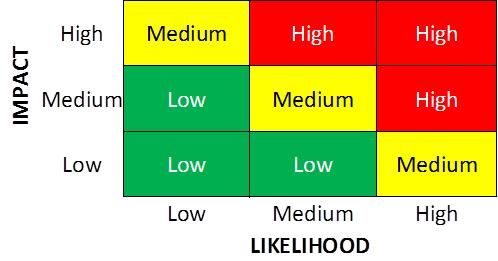
\includegraphics[scale=0.5]{Updated-Risk-Matrix.jpg} % w finalnej prezentacji może się lepiej ułoży
\end{center}


\end{document}
